\chapter{Integral Computation Methods} \label{sec:Chapter4}

In this chapter, the techniques used to compute the integral forms of the normalizing constant in equations (\ref{eq:start_simplex_single_server}), (\ref{eq:start_simplex_inf_server}), and (\ref{eq:multiserver_1}) are described. We will first cover techniques to transform the integral forms of the normalizing constant from an integral over the \(K\)-dimensional simplex, to an integral over \(\mathbb{R}^{K-1}\). Section \ref{sec:logistic_transforms} covers the basic transformations that make this possible, and outlines several characteristics of these transforms. The next section \ref{sec:NC_integral_under_transform}, the transform is applied to the integrals, and Laplace's method is shown to give a good asymptotic approximation to these transformed integrals. Besides that, new results for multi-server networks are derived and presented in section \ref{ssec:multi_server_node_network_results}, and novel results for the integrals under the multiplicative transform are presented in \ref{ssec:mult_transform_results}.
\\\\
Section \ref{sec:MCI} outlines how Laplace's method relates closely to importance sampling of a uni-modal integrand, and how the results from the previous section can be used in the context Monte Carlo integration. The final section \ref{sec:put_all_together} summarizes all the results in this chapter, and brings it together in the context of Monte Carlo integration of the normalizing constant - the Logistic Sampling algorithm. 

\section{Simplex Geometry and Logistic Transforms}\label{sec:logistic_transforms}
In this section we focus on the techniques of transforming the problem of integration of a function over the simplex \(\mathbb{S}^K\) to an integral over the real domain \(\mathbb{R}^{K-1}\)., based on techniques first defined in \cite{Aitchison1982TheData} (nicknamed the logistic transformations). Besides that, certain general properties and identities of these transforms will be introduced, as they will be of use when attempting to compute the integral forms of the normalizing constant (\ref{eq:start_simplex_single_server}), (\ref{eq:start_simplex_inf_server}), and (\ref{eq:multiserver_1}). 

\subsection{Definition of Coordinate Systems and Transforms} \label{sec:transform_def}

In \cite{Aitchison1982TheData}, Aitchison was primarily interested in the analysis of compositional data, these are data whose sample space is the the positive K-dimensional \(\kappa\)-simplex \(\mathbb{S}_{\kappa}^K\). 
\begin{equation*}
    \mathbb{S}_{\kappa}^K = \bigg  \{ \mathbf{u} : \forall u_i > 0, \sum_{i=1}^K u_i = \kappa \bigg \}
\end{equation*}

The difficulty of working with points on the simplex directly \(\mathbf{u}\) included problems with the difficulty of analysing and interpreting correlations in these data, as most tools in probability theory have been made for unconstrained data. The solution was to introduce the log-ratio analysis of components by analyzing the log of the ratios of components, for instance, the log of the ratio of each component over the last component:
\[ x_i = \log \bigg( \frac{u_i}{u_K} \bigg) \]
This is essentially the additive-log-ratio, or additive-logistic transform proposed in \cite{Aitchison1982TheData}, and maps all points on \(\mathbb{S}^K\) to a unique point on \(\mathbb{R}^{K-1}\), and vice versa for the inverse transformation, making it an isomorphic transform. It is one of many transforms proposed in \cite{Aitchison1982TheData}. We can then use this change of coordinates to change the problem of integral on \(\mathbb{S}^K\), to an integral on all of \(\mathbb{R}^{K-1}\).
\begin{equation*}
    \int_{\mathbb{S}^K} f(\mathbf{u}) d \mathbf{u} = \int_{\mathbb{R}^{K-1}} f(\mathbf{x(u)}) \bigg| \frac{\partial \mathbf{u}}{\partial \mathbf{x}} \bigg| d \mathbf{x}
\end{equation*}
\\\\
We will focus on two particular transforms suggested by \cite{Aitchison1982TheData}, namely the multiplicative and additive logistic transforms, and outline some properties when moving between the simplex, and the real domains onto which these transforms map points on the simplex to.
\begin{table}[H]
    \begin{center}
    \begin{tabular}{@{}ll@{}}
    \toprule
    \textbf{Notation} & \textbf{Description} \\ \midrule
        \(\mathbf{u}\)  & Vector representing a point on the unit simplex \(\mathbb{S}^{K}\)   \\
        \(\mathbf{x}^{(A)}\) & A mapped point from the unit simplex onto \(\mathbb{R}^{K-1}\) under the additive transform\\
        \(\mathbf{x}^{(M)}\)  & A mapped point from the unit simplex onto \(\mathbb{R}^{K-1}\) under the multiplicative transform\\ \bottomrule
    \end{tabular}
    \end{center}
    \caption{Notation of relevant coordinate systems}
\end{table}

Both the additive and multiplicative logistic transforms are functions which carry out the following transformation of coordinates:
\[f : \mathbb{R}^{K-1} \rightarrow \mathbb{S}^{K}\]

The additive transform (and inverse) is defined:
\begin{equation}\label{eq:fwd_transform_add}
    u_i = f_{A}(x^{(A)}_i) = 
    \begin{cases}
    e^{x^{(A)}_i} \bigg( 1 + \sum_{k=1}^{i} (e^{x^{(A)}_k}) \bigg)^{-1} & i=1...K-1 \\
    \bigg( 1 + \sum_{k=1}^{i} (e^{x^{(A)}_k}) \bigg)^{-1} & i=K \\
    \end{cases}
\end{equation} 
\begin{equation}\label{eq:inv_transform_add}
    x^{(A)}_i = f_{A}^{(-1)}(u_i) = 
    \log \frac{u_i}{u_K } \quad i=1...K-1
\end{equation} 

The multiplicative transform (and inverse) is defined:
\begin{equation}\label{eq:fwd_transform_mult}
    u_i = f_{M}(x^{(M)}_i) = 
    \begin{cases}
    e^{x^{(M)}_i} \bigg( \prod_{k=1}^{i} (1+e^{x^{(M)}_k}) \bigg)^{-1} & i=1...K-1 \\
    \bigg( \prod_{k=1}^{K-1} (1+e^{x^{(M)}_k}) \bigg)^{-1} & i=K \\
    \end{cases}
\end{equation} 
\begin{equation}\label{eq:inv_transform_mult}
    x^{(M)}_i = f_{M}^{(-1)}(u_i) = 
    \log \frac{u_i}{ 1- \sum_{k=1}^{i} u_k } \quad i=1...K-1
\end{equation} 

The relationship between the two transforms and the simplex can be shown in the diagram below, with their respective Jacobians.

\begin{figure}[H]
\begin{center}
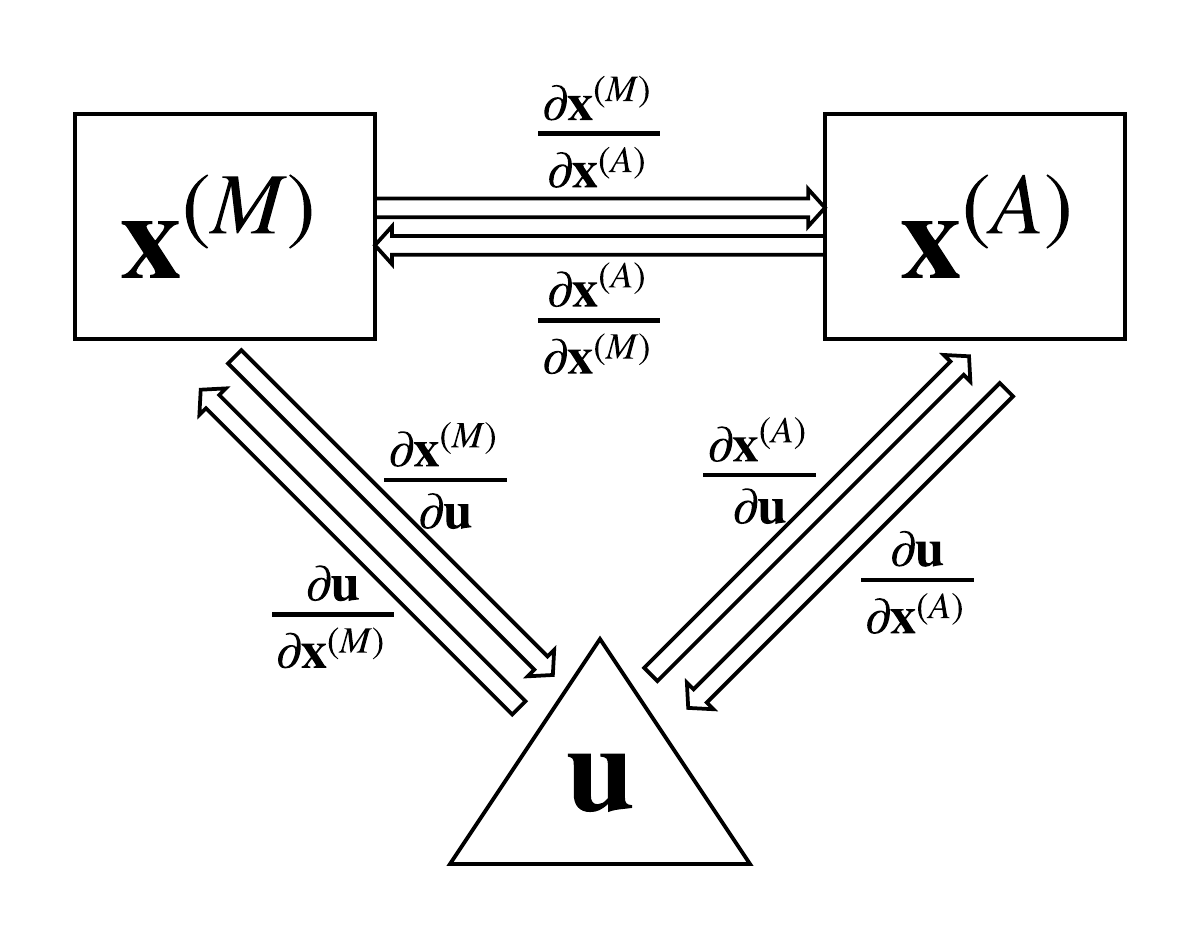
\includegraphics[width=.5\textwidth]{Chap4_ComputationOfIntegral/Coordinate_transformations.png}
\caption{Coordinate transformations and their Jacobians}
\label{fig:coord_transform}
\end{center}
\end{figure}

\begin{table}[H]
    \begin{center}
    \begin{tabular}{@{}lll@{}}
    \toprule
    \textbf{Shorthand} & \textbf{Meaning} & \textbf{Description} \\ \midrule
        \(\mathbf{J_u(x^{A})}\)  &  \({\partial \mathbf{u}}/{\partial \mathbf{x}^{(A)}}\)  & Simplex under additive transform  \\
        \(\mathbf{J_u(x^{M})}\) & \({\partial \mathbf{u}}/{\partial \mathbf{x}^{(A)}}\)  &  Simplex coordinates under Multiplicative transform\\
        \(\mathbf{J_{x^{(M)}}(x^{(A)})}\)  &  \({\partial \mathbf{\mathbf{x}^{(M)}}}/{\partial \mathbf{x}^{(A)}}\)  &  Transform between multiplicative and additive domains\\ \bottomrule
    \end{tabular}
    \end{center}
    \caption{List of Shorthand for Jacobians for coordinate transformations}
\end{table}

Of particular interest to this project are the Jacobians when transforming from \(\mathbf{u}\) coordinates on \(\mathbb{S}^K\) to \(\mathbf{x}^{(A)}\) and \(\mathbf{x}^{(M)}\) coordinates on \(\mathbb{R}^{K-1}\), given by \(\mathbf{J_u(x^{A})}\) and \(\mathbf{J_u(x^{M})}\) respectively. As well as between \(\mathbf{x}^{(A)}\) and \(\mathbf{x}^{(M)}\) given by \(\mathbf{J_{x^{(M)}}(x^{(A)})}\). For \(\mathbf{J_u(x^{A})}\) and \(\mathbf{J_u(x^{M})}\), we are more interested in the determinants of these matrices. \cite{Aitchison1982TheData} gives them as :

\begin{equation}
    |\mathbf{J_u(x^{A})}| = |\mathbf{J_u(x^{M})}| = \prod_{i=1}^K u_i
\end{equation}

On the other hand, we are interested in the explicit form of \(\mathbf{J_{x^{(M)}}(x^{(A)})}\). We show here the derivation of this result, using the chain rule:
\begin{empheq}[box=\mymath]{equation}\label{eq:Jacobian_mult_add}
    \mathbf{J_{x^{(M)}}(x^{(A)})} = \frac{\partial x^{(A)}_i}{\partial x^{(M)}_j} = \frac{\partial x^{(A)}_i}{\partial u_k} \frac{\partial u_k}{\partial x^{(M)}_j}
\end{empheq}
Using the transform between \(x_i^{(A)}\) and \(u_i\) ,  \(x_i^{(A)} = \log \frac{u_i}{u_K}\), and the inverse transform between \(x_i^{(M)}\) and \(u_i\) , equation (\ref{eq:inv_transform_mult}), we get the following.
\\\\
For the first term, \( \frac{\partial x^{(A)}_i}{\partial u_k} \)
\begin{equation}
    \begin{split}
        \frac{\partial x_i}{\partial u_k} & = \frac{\partial}{\partial u_k} \bigg( \log \frac{u_i}{u_K} \bigg)\\
        & =  \frac{u_K}{u_i} \bigg( \frac{1}{u_K} \delta_{ik}  - \frac{u_i}{u_K} \delta_{Kk} \bigg) \\
    \end{split}
\end{equation}

For the second term \( \frac{\partial u_k}{\partial x^{(M)}_j} \), it is zero for when \( j > k\), and otherwise:
\begin{equation}
    \begin{split}
        \frac{\partial u_k}{\partial x^{(M)}_j} & = \frac{\partial}{\partial x^{(M)}_j} \bigg( \frac{e^{x^{(M)}_k}}{\prod_{p=1}^k 1 + e^{x^{(M)}_p}} \bigg) \\
        & = \delta_{kj} \frac{e^{x_k^{(M)}} }{\prod_{p=1}^k 1 + e^{x^{(M)}_p} } + 
        \frac{ e^{x_k^{(M)}} e^{x_j^{(M)}} } { \bigg( 1 + e^{x^{(M)}_j} \bigg) \bigg(\prod_{p=1}^k 1 + e^{x^{(M)}_p} \bigg) }\\
        &= \delta_{kj} u_k + u_k \beta_j(\mathbf{u})
    \end{split}
\end{equation}
Where \(\beta_j(\mathbf{u})\) is defined as:
\[ \beta_j(\mathbf{u}) = \begin{cases} 
u_j & j=1 \\
\frac{u_j}{1 - \sum^{j-1}_{p=1} u_p} & j>1
\end{cases}\]

It is also worth mentioning that while \(\mathbf{J_u(x^{A})}\), \(\mathbf{J_u(x^{M})}\), and \(\mathbf{J_{x^{(A)}}(x^{M})}\) have been expressed above in terms of simplex coordinates \(\mathbf{u}\), they can be expressed equivalently in \(\mathbf{x}^{(A)}\) and \(\mathbf{x}^{(M)}\) without loss of generality, simply by applying the coordinate transforms (\ref{eq:fwd_transform_add}) and (\ref{eq:fwd_transform_mult}).

\subsection{Identities for Functions when Switching Transforms}
The aim of this section is to establish some general identities and properties of functions on the simplex, and some identities for the function under different transformations (namely the additive and multiplicative transforms), and moving between different transformations.
\\\\
Firstly, it should be noted that a function \(g\) defined over the \(K\)-dimensional real space \(\mathbb{R}^K\), can be defined over a \(K+1\)-dimensional simplex \(\mathbb{S}^{K+1}\) as \(g'\), either by applying the logistic additive transform, or logistic multiplicative transform, and vice versa. Take for example the function below defined over \(\mathbb{R}^K\), in terms of \(\mathbf{x}^{(M)}\).
\[g(\mathbf{x}^{(M)}) = g(f_M^{-1}(\mathbf{u})) = g'(\mathbf{u})\]

Here we will simply use \(g(\mathbf{x}^{(M)}) = g(\mathbf{u})\) to indicate this change in transformation as shorthand. Now, given this fact, we can make some statements about the first and second derivatives of these functions, when defined on different transformed domains.
\\\\
When a function \(g(\mathbf{u})\) can be defined in terms of \(\mathbf{x}^{(M)}\) as well as \(\mathbf{x}^{(A)}\), then its derivative with respect to \(\mathbf{x}^{(M)}\) and \(\mathbf{x}^{(A)}\) have the following relationship. Using Einstein notation, and the chain rule:
\begin{empheq}[box=\mymath]{equation} \label{eq:first_derivatives}
    \begin{split}
    \frac{ \partial g(\mathbf{x}^{(M)}) }{\partial \mathbf{x}^{(M)} }
    & = \frac{ \partial g(\mathbf{u}) }{\partial u_k } \frac{ \partial u_k }{\partial x_i^{(M)} }\\
    & = \frac{ \partial g(\mathbf{x}^{(A)}) }{\partial x_j^{(A)} } \frac{ \partial x_j^{(A)} }{\partial x_i^{(M)} }
    \end{split}
\end{empheq}

For the second derivative (Hessian), using the chain rule again, this becomes:
\begin{empheq}[box=\mymath]{equation}\label{eq:second_derivatives}
    \begin{split}
        \frac{ \partial^2 g(\mathbf{x}^{(M)}) }{\partial \mathbf{x}^{(M)2} }
        & = \frac{ \partial }{\partial x^{(M)}_i} \bigg[ \frac{ \partial g(\mathbf{x}^{(A)}) }{\partial x^{(A)}_p } \frac{ \partial x^{(A)}_p }{\partial x^{(M)}_j } \bigg]\\
        & = \frac{ \partial^2 g(\mathbf{x}^{(A)})}{\partial x^{(A)}_q \partial x^{(A)}_p } \frac{ \partial x^{(A)}_p }{\partial x^{(M)}_j } \frac{ \partial x^{(A)}_q }{\partial x^{(M)}_i } 
        + \frac{ \partial^2 x^{(A)}_p }{\partial x^{(M)}_i \partial x^{(M)}_j}  \frac{ \partial g(\mathbf{x}^{(A)}) }{\partial x^{(A)}_p }\\
    \end{split}
\end{empheq}

In the following theorem, we describe and prove the relationship between the stationary points of both transforms.
\begin{theorem} \label{theorem:stat_point_mult_add}
    If \( \hat{\mathbf{x}}^{(A)} \) is a stationary point for the function \(g(\mathbf{x}^{(A)})\), i.e. \( \frac{\partial g(\hat{\mathbf{x}}^{(A)})}{\partial \mathbf{x}^{(A)}} = \mathbf{0}\), and \(\hat{\mathbf{u}} = f_A^{-1}(\hat{\mathbf{x}}^{(A)})\), then \(\hat{\mathbf{x}}^{(M)} = f_M( \hat{\mathbf{u}} )\) is a stationary point to \(g(\mathbf{x}^{(M)})\) , or \( \frac{\partial g(\hat{\mathbf{x}}^{(M)})}{\partial \mathbf{x}^{(M)}} = \mathbf{0}\).
    Furthermore, if the transform between \(\mathbf{x}^{(A)}\) and \(\mathbf{x}^{(M)}\) is nonsingular at the stationary points, then a stationary point for \(g(\mathbf{x}^{(M)})\) is also a stationary point for \(g(\mathbf{x}^{(A)})\).
\end{theorem}

\begin{proof}
    We can see this by examining the first derivatives for the additive and multiplicative mappings. Using \ref{eq:first_derivatives}, we can write: 
    \begin{equation} \label{eqn:stat_point}
        \mathbf{m} = \mathbf{J}^T  \mathbf{a} 
    \end{equation} 
    Where the terms mean: 
    \begin{itemize}
        \item \( \mathbf{m} = \frac{\partial g(\mathbf{x}^{(M)})}{\partial \mathbf{x}^{(M)}} \) - the vector of first derivative of \(h\) w.r.t to \(\mathbf{x^{(M)}}\)
        \item \( \mathbf{a} = \frac{\partial g(\mathbf{x}^{(A)})}{\partial \mathbf{x}^{(A)}} \) - the vector of first derivative of \(h\) w.r.t to \(\mathbf{x^{(A)}}\)
        \item \( \mathbf{J} = \mathbf{J}_{\mathbf{x}^{(M)}}(\mathbf{x}^{(A)}) \) - the Jacobian between \(\mathbf{x^{(A)}}\) and \(\mathbf{x^{(M)}}\)
    \end{itemize}
    
    Without any loss of generality, all three terms above can be expressed in simplex coordinates \(\mathbf{u}\). To solve for a stationary point \(\mathbf{\hat{u}}^{(A)} = f_A^{-1}(\hat{\mathbf{x}}^{(A)})\), under the additive coordinate transformation, we equate:
    \begin{equation} \label{eqn:add_stat_point} 
        \mathbf{a}(\mathbf{\hat{u}}^{(A)}) = \frac{\partial g(\mathbf{\hat{u}}^{(A)})}{\partial \mathbf{x}^{(A)}} = \mathbf{0} 
    \end{equation}
    Similarly for a stationary point under the multiplicative transform \(\mathbf{\hat{u}}^{(M)} = f_A^{-1}(\hat{\mathbf{x}}^{(M)}) \) : 
    \begin{equation} \label{eqn:mult_stat_point} 
        \mathbf{m}(\mathbf{\hat{u}}^{(M)}) = \frac{\partial g(\mathbf{\hat{u}}^{(M)})}{\partial \mathbf{x}^{(M)}} = \mathbf{0} 
    \end{equation}
    
    However, we can also show that \(\mathbf{\hat{u}}^{(A)}\) is also a solution to (\ref{eqn:mult_stat_point}), by using (\ref{eqn:stat_point}):
    \begin{equation}
        \begin{split}
            \mathbf{m}(\mathbf{\hat{u}}^{(A)}) & = \mathbf{J}^T (\mathbf{\hat{u}}^{(A)})  \mathbf{a} (\mathbf{\hat{u}}^{(A)}) \\ 
            & = \mathbf{J}^T (\mathbf{\hat{u}}^{(A)})  \mathbf{0}\\
            & = \mathbf{0}
        \end{split}
    \end{equation}
    
    If the transform between the coordinate systems \(\mathbf{x}^{(A)}\) and \(\mathbf{x}^{(M)}\) is nonsingular at the stationary point, then by the inverse function theorem, the Jacobian of the inverse transform \(\mathbf{J_{x^{(A)}}(x^{(M)})}\) is the inverse of the Jacobian of the forward transform \(\mathbf{J_{x^{(M)}}(x^{(A)})}^{-1}\). We can then re-write (\ref{eqn:stat_point}) as:
    \begin{equation*}
        \mathbf{a} = \mathbf{(J^{-1})^T} \mathbf{m}
    \end{equation*}
    Then we can make a symmetric argument to conclude that if \(\mathbf{\hat{u}}^{(M)}\) is a stationary point of \(g(\mathbf{x}^{(M)})\), then it is also a stationary point of \(g(\mathbf{x}^{(A)})\).
\end{proof}

Given these identities, we can now use them to derive the integral form of the integrals (\ref{eq:start_simplex_single_server}), (\ref{eq:start_simplex_inf_server}), and (\ref{eq:multiserver_1}), over \(\mathbb{R}^K\).
 

\section{Normalizing Constant Integrals under Transform}\label{sec:NC_integral_under_transform}

In this section, we derive the integral forms of the normalizing constant, after applying the transformation functions defined in section \ref{sec:transform_def}, to the integrals ((\ref{eq:start_simplex_single_server}), (\ref{eq:start_simplex_inf_server}), and (\ref{eq:multiserver_1})). The properties of this transformed integral and their implications on the methods of computation will also be covered in detail. 
\\\\
Sections \ref{ssec:single_server_results} - \ref{ssec:multi_server_node_network_results} will focus on deriving the integral form of the normalizing constant, after applying the additive logistic transformation (\ref{eq:fwd_transform_add}), for single server node networks, single and infinite server node networks, and multi-server node networks. Section \ref{ssec:mult_transform_results} will then move on the deriving results using the multiplicative logistic transform (\ref{eq:fwd_transform_mult}), on single server networks, as well as single and infinite server networks.
\\\\
Important results will be presented in highlighted boxes, for the ease of the reader.
\subsection{Preliminaries}
The integral forms for the normalizing constant were first derived by \cite{Casale2017AcceleratingMethods} to be used with Laplace's method of integration. This method is used when an integral of the form shown in equation(\ref{eq:laplace_int}), which is the form of the simplex integrals ((\ref{eq:start_simplex_single_server}), (\ref{eq:start_simplex_inf_server}), and (\ref{eq:multiserver_1})) after applying the logistic transformations (both additive and multiplicative).
\begin{equation} \label{eq:laplace_int}
    I = \int_{\mathbb{R}^{K-1}} g(\mathbf{x}) e^{-\lambda f(\mathbf{x})} d\mathbf{x}
\end{equation}
satisfies the following conditions.
\begin{itemize}[noitemsep]
    \item Condition 1: \(I\) exists and is finite
    \item Condition 2: \(f(\mathbf{x})\)  attains a unique minimum in the interior of the integration domain
    \item Condition 3: \(g(\mathbf{x})\) and \(f(\mathbf{x})\) are smooth
\end{itemize}

Given this conditions, Laplace's method approximates the integral (\ref{eq:laplace_int}) as \cite{Azevedo-Filho1994LaplacesVariables}:
\[e^{- \lambda g(\mathbf{\hat{x}}) } h(\mathbf{\hat{x}}) { \frac{(2\pi)^{(K-1)/2}}{|\mathbf{A}|^{1/2}} } + \epsilon \]

Where \(\mathbf{\hat{x}}\) is the stationary point at which \(h(\mathbf{x})\) attains its minimum value, and \(\mathbf{A}\) is the hessian of \(h(\mathbf{x})\) at \(\mathbf{\hat{x}}\). Furthermore, \(\epsilon \sim O(N^{-1})\). Essentially, Laplace's method approximates \(e^{-\lambda f(\mathbf{x})}\) as a Gaussian PDF, with mean \(\boldsymbol{\mu} = \mathbf{\hat{x}}\), and inverse covariance \(\boldsymbol{\Sigma}^{-1} = \mathbf{A}\).
\\\\
In order for Laplace's method to be applicable as \(N \rightarrow + \infty\), the stationary point of the transformed integrand must remain in the interior of the integration domain of the simplex. Besides that, the hessian of the integrand must also be symmetric and positive-definite at the stationary point. To enforce these conditions for all \(N\), \cite{Casale2017AcceleratingMethods} introduces a novel perturbation of the model, by adding \(K\) additional classes of jobs that permanently reside in one node per class. Each class is assigned \(\epsilon N\) jobs, \(\epsilon > 0\), and each job places a unit service demand each visit. The perturbed normalizing constant can then be written:
\begin{empheq}[box=\mymath]{equation}
    G_{\boldsymbol{\theta}}^{\epsilon}(\mathbf{N}) = 
    \frac{\Gamma(\eta_{\epsilon}(N))}{\Gamma(1+\epsilon N))^K \prod_{i=1}^K N_i!} I_{\epsilon}(\mathbf{N})
\end{empheq}
Where \(I_{\epsilon}(\mathbf{N})\) take the following forms for single server node-networks:
\begin{equation}\label{eq:perturb_single_server_integral}
    I_{\epsilon}(\mathbf{N}) =  \int_{\Delta_K} \prod_{i=1}^K u_i^{\epsilon N} \prod_{r=1}^R \bigg( \sum_{k=1}^K \theta_{kr} u_k \bigg)^{N_r} d\mathbf{u}
\end{equation}
And for networks with infinite and single server nodes:
\begin{equation}\label{eq:perturb_inf_server_integral}
    I_{\epsilon}(\mathbf{N}) =  
    (\Gamma(\eta_{\epsilon}(N)))^{-1}
    \int_{\mathbb{R}^K_+} e^{-v} v^{K(1+\epsilon N)-1} \int_{\Delta_K} 
    \prod_{i=1}^K u_i^{\epsilon N} \prod_{r=1}^R \bigg( \sigma_r + v\sum_{k=1}^K \theta_{kr} u_k \bigg)^{N_r}
    d \mathbf u dv
\end{equation}
And \(\eta_{\epsilon}(N) = N + K(1+\epsilon N)\).
\\\\
While the main focus of this project does not use Laplace's method to compute the normalizing constant, the conditions for the use of this method prove useful for the use of the Monte Carlo integration technique, and importance sampling, as will be covered in \ref{sec:MCI}. 

\subsection{Results for Single Server Node Networks}\label{ssec:single_server_results}

We first apply the additive logistic transformation (\ref{eq:fwd_transform_add})  to the perturbed integral for single server networks (\ref{eq:perturb_single_server_integral}), with Jacobian:
\[ \bigg | \frac{\partial \mathbf{u}}{\partial \mathbf{x}} \bigg |  = \prod_{i=1}^K u_i = \prod_{i=1}^{K-1} e^{x_i} \bigg( 1 + \sum_{k=1}^{K-1}e^{x_k} \bigg)^{-K}\]
to obtain an integral of the form:
\begin{equation}\label{eq:integral_form_single_server}
    I_{\epsilon}(\mathbf{N}) = \int_{\mathbb{R}^{K-1}} e^{-N h(\mathbf{x})} d \mathbf{x}
\end{equation}

Where the exponent \(-N h(\mathbf{x})\) takes the form: 
\begin{empheq}[box=\mymath]{equation}\label{eq:log_integrand_single_server}
    -N h(\mathbf{x}) = \sum_{i=1}^{K-1} (1 + \epsilon N) x_i 
    + \sum_{r=1}^R N_r \log \bigg( \theta_{Kr} + \sum_{k=1}^{K-1} \theta_{kr} e^{x_k} \bigg) - 
    \eta_{\epsilon}(N) \log \bigg( 1+ \sum_{k=1}^{K-1} e^{x_k} \bigg)
\end{empheq}

It can be equivalently expressed in simplex coordinates:
\begin{equation}
    -N h(\mathbf{u}(\mathbf{x})) =  \sum_{r=1}^R N_r \log \bigg( \sum_{i=1}^K \theta_{kr} u_k \bigg) + 
    \sum_{k=1}^{K-1} (1 + \epsilon N) \log u_k
\end{equation}
Note that \(h(\mathbf{x})\) is smooth and infinitely differentiable, and has constant order with respect to \(N\), satisfying condition 3 for Laplace's method. 

\begin{lemma}
    The solution to the following system of \(K-1\) nonlinear equations is the stationary point of \(h(\mathbf{x})\):
    \begin{empheq}[box=\mymath]{equation}\label{eq:single_server_stat_pt_equation}
        u_i = \eta_{\epsilon}^{-1}(N) \bigg( 1 + \epsilon N + \sum_{r=1}^R \xi_r (\mathbf{u}) \theta_{ir} u_i  \bigg) \quad \forall i = 1, ... , K-1
    \end{empheq}
    With \(\xi_r (\mathbf{u}) = N_r (\sum_k^K \theta_{kr} u_k)^{-1} \). 
\end{lemma}

To derive the stationary point equations for \(h(\mathbf{x})\), we first compute the derivative of \(-N h(\mathbf{x})\) and equate to zero:
\begin{equation*}
    \begin{split}
        \frac{\partial h(\mathbf{x})}{\partial x_i} = & \frac{\partial h(\mathbf{u})}{\partial u_j} \frac{\partial u_j}{\partial x_i}\\
        & = \sum_{j=1}^K \bigg[ \bigg( \theta_{jr} \sum_{r=1}^R N_r \bigg( \sum_{k=1}^K \theta_{kr} u_k \bigg)^{-1} + 
        u_j (1 + \epsilon N) \bigg) \bigg( \delta_{ji} u_i - u_i u_j \bigg) \bigg]\\
        & = \bigg( - \eta_{\epsilon}(N) u_i +  1 + \epsilon N + \sum_{r=1}^R \xi_r (\mathbf{u}) \theta_{ir} u_i  \bigg) = 0
    \end{split}
\end{equation*}


\begin{lemma}
    The hessian of \(h(\mathbf{x})\) at the stationary point \(\mathbf{\hat{x}}\), \(\mathbf{A}\) is given by: 
    \begin{empheq}[box=\mymath]{equation}\label{eq:single_server_hessian_exp}
            A_{ij} = 
            \begin{cases}
                -\sum_{\substack{h=1 \\ h \neq i}}^K A_{ih} & i = j \\
                \bigg( \sum_{r=1}^R \frac{\xi_r^2(\mathbf{\hat{u}}))}{N_r} \theta_{ir}\theta_{jr}  - \eta_{\epsilon}(N) \bigg) \hat{u}_i \hat{u}_j & i \neq j \\
            \end{cases}
    \end{empheq}
\end{lemma}

At the stationary point \(\mathbf{\hat{u}}\), to obtain the hessian in terms of simplex coordinates we can do:
\begin{equation*}
    \begin{split}
        \frac{\partial^2 h(\mathbf{\hat{x}})}{\partial x_i \partial x_j} & = \frac{\partial }{\partial u_q} \bigg[ \frac{\partial h(\mathbf{\hat{x}})}{\partial x_j} \bigg] \frac{\partial u_q}{\partial x_i}\\
        & = \sum_{q=1}^K \bigg[ \delta_{qj}u_j (\delta_{qi}u_i - u_i u_q) \bigg( -\eta_{\epsilon}(N) + \theta_{jr} \theta_{qr} \sum_{r=1}^R \frac{\xi^2_r(\mathbf{\hat{u}})}{N_r} \bigg) \bigg]
    \end{split}
\end{equation*}
The result then follows by simplifying.

\subsection{Satisfying the Conditions of Laplace's Method} \label{ssec:laplaces_method_conditions}

By following the argument presented in \cite{Casale2017AcceleratingMethods}, we will now use the results (\ref{eq:single_server_stat_pt_equation}) and (\ref{eq:single_server_hessian_exp}) to show that the integral for single-server networks under the additive transform satisfies the requirements for Laplace's method.
\\\\
\textit{\large{Condition 1: Existence and Finiteness of \(I_{\epsilon}(N)\)}}
\\\\
Since the logistic transformation does not affect existence and finiteness of \(I_{\epsilon}(N)\), it is sufficient to evaluate these properties on the original form of \(I_{\epsilon}(N)\), on the simplex (\ref{eq:perturb_single_server_integral}). The integrand of (\ref{eq:perturb_single_server_integral}) is finite at all points in the simplex, \(0 \leq u_i \leq  1 , \forall i\), for finite \(\epsilon, N\), and \(\epsilon > 0, N > 0\). The volume of the simplex is also constant irrespective of the value of \(N\), which will result in a finite intergal.
\\\\
\textit{\large{Condition 2: Unique Stationary Point of Integrand \(e^{N h(\mathbf{x})}\)}}
\\\\
Using the stationary point equation \ref{eq:single_server_stat_pt_equation}, we seek to show that the system admist a unique solution \(\mathbf{\hat{u}}\). Moreover we also show that if \(\epsilon > 0\), then \(\mathbf{\hat{u}} \in \Delta_{K,N}^{\epsilon} \subset \Delta_K\) for all \(N>0\), with
\[ \Delta_{K,N}^{\epsilon} = \{ \mathbf{u} : \mathbf{u} \in \Delta_K, u_i \geq (1+\epsilon N )\eta_{\epsilon}^{-1}(N), \forall i  \} \]
Roughly speaking, for \(\epsilon N > 0\) the above condition ensures that there are no \(\hat{u}_i\) that will take on the extreme values of \(0\) or \(1\), resulting in the stationary point in \(\mathbb{R}^{K-1}\), \(\mathbf{\hat{x}}\) to be located at plus or minus infinity:
\[ \mathbf{\hat{x}} = \bigg[ \log \bigg(\frac{\hat{u}_1}{\hat{u}_K} \bigg), ... , \log \bigg(\frac{\hat{u}_{K-1}}{\hat{u}_K}\bigg)  \bigg]\]
To begin, we prove that it is indeed the case that \(\mathbf{\hat{u}} \in \Delta_{K,N}^{\epsilon}\). Let us consider a point \(\mathbf{u}^{(n)} \in \Delta_K\), \(n \in \mathbb{N}\), and the continuous mapping
\begin{equation}\label{eq:fixed_point_simplex}
    u_i^{(n+1)} = \eta_{\epsilon}^{-1}(N) \bigg( 1 + \epsilon N + \sum_{r=1}^R \xi_r (\mathbf{u}^{(n)}) \theta_{ir} u_i^{(n)}  \bigg)
\end{equation}
Since \(\Delta_K\) is convex, non-empty and compact, (\ref{eq:fixed_point_simplex}) must have a solution \(\mathbf{\hat{u}} \in \Delta_K\) and this is also a solution of (\ref{eq:single_server_stat_pt_equation}) by definition. We can show by contradiction that (\ref{eq:fixed_point_simplex}) has no solution in \(\Delta_K \backslash \Delta_{K,N}^{\epsilon}\). Assuming that there exists a solution \(\mathbf{\hat{u}}'\) to (\ref{eq:fixed_point_simplex}) such that \(\mathbf{\hat{u}}' \in \Delta_K, \hat{u}_i' < (1+\epsilon N )\eta_{\epsilon}^{-1}(N)\), then plugging \(u_i'\) into the \(i\)-th equation of (\ref{eq:fixed_point_simplex}) will render it infeasible, since this will reduce to:
\[v_i = 1 + \epsilon N + v_i \eta_{\epsilon}(N)^{-1} \sum_{r=1}^R \xi_r (\mathbf{u}^{(n)}) \theta_{ir}\]
Where \(v_i = u_i' \eta_\epsilon (N)\) and it is required that \(v_i < 1 + \epsilon N\). It becomes obvious that a solution to this is impossible since it is always the case that \(\sum_{r=1}^R \xi_r (\mathbf{u}^{(n)}) \theta_{ir} > 0\) and \(v_i > 0\).
\\\\
To prove the uniqueness of \(\mathbf{\hat{u}}\), we focus on \(\Delta_{K,N}^{\epsilon}\), since no solutions exist outside this subdomain. Now it can be proven that \(\mathbf{\hat{u}}\) is a solution to (\ref{eq:single_server_stat_pt_equation}) if and only if it is a solution to the following nonlinear program:
\begin{equation}
    \min_{\mathbf{u} \in \Delta_{K,N}^\epsilon} \sum_{i=1}^{K-1} \frac{u_i^2}{2} - \eta_{\epsilon}^{-1}(N)
        \bigg( (1 + \epsilon N) \sum_{i=1}^{K-1} u_i + \sum_{r=1}^R N_r \log \bigg(  \sum_{k=1}^K \theta_{kr} u_k \bigg)  \bigg)
\end{equation}
With first-order Karush-Kuhn-Tucker(KKT) conditions:
\begin{gather*}
    -u_i + \eta_{\epsilon}^{-1}(N) \bigg( 1 + \epsilon N + \sum_{r=1}^R \xi_r \theta_{ir} u_i \bigg) = \lambda + \mu_i \\
    \sum_{k=1}^K u_k = 1 \\
    u_i \mu_i = 0\\
    \eta_{\epsilon}(N) u_i \geq 1 + \epsilon N\\
    \mu_i \geq 0\\
\end{gather*}
For all \(i = 1...K-1\). A feasible solution in \(\Delta_{K,N}^{\epsilon}\) requires that \(\mu_i = 0\) for all i. It is possible also to verify that the objective is strictly convex over \(\Delta_{K,N}^{\epsilon}\), being the sum of functions that are convex and strictly convex over the domain. Given this condition, the KKT conditions admit a unique solution, which must be \(\mathbf{\hat{u}}\) since this is feasible when \(\lambda = 0\). This allows us to conclude that \ref{eq:single_server_stat_pt_equation} has a unique solution \(\mathbf{\hat{u}}\) in \(\Delta_{K,N}^{\epsilon}\).
\\\\
\textit{\large{Condition 2.5: Positive Hessian Determinant of \(\mathbf{A}\)}}
\\\\
Let \(\mathbf{A} = [A_{ij}] , i,j = 1,...,K-1\), be the Hessian of \(Nh(\mathbf{\hat{x}})\), evaluated at the stationary point \(\mathbf{\hat{x}}\). This is given by (\ref{eq:single_server_hessian_exp}). For any \(\epsilon > 0\), there exists a \(0 < \delta < (N+K)^{-1} \) such that:
\[ \sum_{k=1}^{K} \theta_{kr}\hat{u}_k > \delta \max_k \theta_{kr}\]
And we can simply choose \(\epsilon\) to be :
\[\epsilon > \frac{R}{KN} \frac{(\max_{k,r} \theta_{kr}^2) (\max_r N_r)}{\delta^2 (\min_r \max_k \theta_{kr})} \]
Which is a finite value (\(\epsilon < \infty\)), and will always guarantee positive off-diagonal entries for \(\mathbf{A}\). This implies that:
\begin{equation}
    \mathbf{Q} = - \begin{bmatrix} 
        \mathbf{A} & \mathbf{a}_K^T \\
        \mathbf{a}_K & A_{KK} \\
    \end{bmatrix}
\end{equation}
with \(\mathbf{a}_K = (A_{1K}, ... , A_{K-1,K})\) is an irreducible infinitesimal generator. Being \(- \mathbf{A}\) the principal sub-matrix of an irreducible generator, it is negative definite and thus \(\mathbf{A}\) is positive definite, implying \(|\mathbf{A}| > 0\).
\\\\
\textit{\large{Final Result of Laplace's Expansion}}
\\\\
Conditions 2 and 2.5 imply that \(h(\mathbf{x})\) attains a unique minimum in \(\mathbb{R}^{K-1}\) for some finite value of \(\epsilon\). Conditions 1, 2, and 2.5 taken together thus completes the proof that \(I_\epsilon (N)\) under the additive logistic transform satisfies all of the conditions required for Laplace's method to be used as an asymptotic expansion. Applying Laplace's method to the evaluation of \(I_\epsilon(N)\), we obtain the expansion:
\begin{empheq}[box=\mymath]{equation}
    \begin{split}
        I_\epsilon(N)  & = \sqrt{\frac{(2 \pi)^{K-1}}{\det(\mathbf{A})}}  e^{-N h(\mathbf{\hat{x}})} + O(N^{-1}) \\
        & = \sqrt{\frac{(2 \pi)^{K-1}}{\det(\mathbf{A})}} \prod_{r=1}^R \bigg( \sum_{k=1}^K \theta_{kr} \hat{u}_k \bigg)^{N_r} \prod_{i=1}^K \hat{u}_i^{1 + \epsilon N}
    \end{split}
\end{empheq}

While not the ultimate aim of this project, the validity of using Laplace's method has great impact on the effectiveness of the use of the Monte Carlo integration technique to evaluate \(I)\epsilon (N)\). Furthermore, the results derived here will prove very useful for Monte Carlo integration. This will be covered in detail in section \ref{sec:MCI}.

\subsection{Results with Infinite Server Node Networks}\label{ssec:infinte_server_networks_results}

Given the more complicated nature of the integral (\ref{eq:start_simplex_inf_server}), it is difficult to scale the parameters, as was done in the single-server case, and thus it is difficult to confirm the asymptotic validity of Laplace's method. Thus, in methods with infinte servers, \cite{Casale2017AcceleratingMethods} proposed Laplace's method only as a sub-asymptotic heuristic. 
\\\\
A similar form of the integral is derived by applying the additive tranform to the simplex coordinates \(\mathbf{u}\), as well as a change of variable \(x_0 = \log (v)\). Similar results on the stationary point of the integrand and the Hessian matrix is obtained, and Laplace's method will be used to approximate \(I_\epsilon(N)\), for \(N < \infty\). Again, these methods will prove useful in the derivation of results for use in Monte Carlo integration.
\\\\
Applying the transformation, \(I_\epsilon(N)\) takes the form:
\begin{equation}\label{eq:integral_form_infinite_server}
    I_\epsilon(N) = \int_{\mathbb{R}^K} b_N e^{-N h_N(\mathbf{x})} d \mathbf{x}
\end{equation}

Where \(\mathbf{x} = (x_0, x_1, ..... x_{K-1})\), and \(b_N = (\Gamma(\eta_\epsilon(N)))^{-1}\), and:
\begin{empheq}[box=\mymath]
    {equation}\label{eq:log_integrand_infinite_server}
    \begin{split}
        -N h(\mathbf{x}) & = - e^{x_0} + K(1+\epsilon N) x_0 \\
        & + \sum_{r=1}^R \log \bigg( \sigma_r + e^{x_0} \theta_{Kr} + \sum_{k=1}^{K-1}e^{x_k} (\sigma_r + \theta_{kr} e^{x_0}) \bigg) \\
        & + (1 + \epsilon N) \sum_{k=1}^{K-1} x_k - \eta_\epsilon(N) \log \bigg( a + \sum_{k=1}^{K-1} e^{x_k} \bigg)
    \end{split}
\end{empheq}

Where we now have one extra dimension of integration, \(K\), as opposed to \(K-1\) dimensions in the case without infinte serves, owing to the fact that we have introduced an extra variable \(v\). 

\begin{lemma}
    The solution of the following set of nonlinear equations gives the stationary point for the log integrand in (\ref{eq:log_integrand_infinite_server}):
    \begin{empheq}[box=\mymath]{equation} \label{eq:inf_server_stat_point}
        \begin{split}
            u_i & = \eta_{\epsilon}^{-1}(N) \bigg( 1 + \epsilon N + \sum_{r=1}^R \xi_r (\mathbf{u}, v) (\sigma_r + v \theta_{ir}) u_i \bigg) \quad \forall i = 1.. K-1 \\
            v & = \eta_\epsilon(N) + 1 - \sum_{r=1}^R \xi_r(\mathbf{u},v) \sigma_r
        \end{split}
    \end{empheq}
    Where \(\xi_r(\mathbf{u}, v) = N_r (\sigma_r + v \sum_{k=1}^K \theta_{kr}u_k)^{-1}\). 
\end{lemma}

The above result is obtained by setting the derivative of the integrand \(h(\mathbf{x})\) to zero:
\begin{equation*}
    \begin{split}
        \frac{\partial h(\mathbf{x})}{\partial x_i} = & \frac{\partial h(\mathbf{u})}{\partial u_j} \frac{\partial u_j}{\partial x_i} + 
        \frac{\partial h(\mathbf{u})}{\partial v} \frac{\partial v}{\partial x_i} \\
        & = \bigg((1 + \epsilon N)u_i^{-1} + u_i \sum_{r=1}^R \xi_r(\mathbf{u}, v) (\sigma_r + v \theta_{ir})\bigg)\bigg( \delta_{ji}u_i - u_i u_j \bigg) \\
        &+ \delta_{0i}\bigg( v(N - 1) + K(1+\epsilon N) \bigg) = 0 \quad \forall i = 1 ... K-1
    \end{split}
\end{equation*}


For the hessian \(\mathbf A \in \mathbb{R}^{K \times K}\), matrix at the stationary point \((\mathbf{\hat{u}}, \hat{v})\), we proceed in in a similar vein to section \ref{ssec:single_server_results} in its derivation. 
\begin{lemma}
    Defining \(\tilde{\theta}_{kr} = \sigma_r + \hat{v} \theta_{ir}, \forall k,r\), the entries of \( \mathbf{A} = [A_{ij}]\) are given by:
    \begin{empheq}[box=\mymath]{equation}\label{eq:inf_server_hessian}
        \begin{split}
            A_{ii} & = \sum_{h \neq i} A_{ih} \quad \forall i = 1 ... K-1\\
            A_{ij} & = \bigg[ \sum_{r=1}^R \bigg( \frac{\xi_r^2(\mathbf{\hat{u}} , \hat{v})}{N_r} \tilde{\theta}_{ir} \tilde{\theta}_{jr} \bigg) \eta_\epsilon(N) \bigg] \hat{u}_i \hat{u}_j \quad \forall i,j = 1 ... K-1 , i \neq j\\
            A_{00} & = \hat{v} \bigg[ 1 - \sum_{r=1}^R \frac{\xi_r^2(\mathbf{\hat{u}} , \hat{v})}{N_r} \sigma_r \bigg( \sum_{k=1}^K \theta_{kr} \hat{u}_k \bigg) \bigg] \\
            A_{i0} & = A_{0i} = \hat{v} \hat{u}_i \sum_{r=1}^R \bigg[ \frac{\xi_r^2(\mathbf{\hat{u}} , \hat{v})}{N_r} \hat{\theta}_{ir} \bigg( \sum_{k=1}^K \theta_{kr} \hat{u}_k \bigg) - \xi_r(\mathbf{\hat{u}} , \hat{v}) \theta_{ir} \bigg]
        \end{split}
    \end{empheq}
\end{lemma}

As mentioned before, similar conditions for Laplace's method cannot be proven formally for the above results. Nevertheless, it provides the required results for a Laplace-type approximation, and has been proven to work in multiple numerical experiments, both in \cite{Casale2017AcceleratingMethods}, as well as in this project (see \ref{sec:overview_experiments}). The resulting expansion would be:
\begin{equation}
    I_\epsilon(N) \approx \frac{e^{-\hat{v}} \hat{v}^{K(1+\epsilon N)}}{\Gamma(\eta_\epsilon(N)} \sqrt{ \frac{(2 \pi)^K}{|\mathbf{A}|} } \prod_{r=1}^R \bigg( \theta_r + \hat{v} \sum_{k=1}^K \theta_{kr} \hat{u}_k \bigg)^{N_r} \prod_{k=1}^K \hat{u}_k^{1 + \epsilon N}
\end{equation}

Of particular interest in this section are equations (\ref{eq:inf_server_stat_point}) and (\ref{eq:inf_server_hessian}), which are results that are important for the Monte Carlo integration method presented in this project.

\subsection{Results for  Multi-server Node Networks} \label{ssec:multi_server_node_network_results}
In this project, we introduce novel results for the multi-server node network case, applying the additive transform to the integral (\ref{eq:multi_server_NC}), and deriving results similar to those of the single-server networks as well as infinite-server networks.
\\\\
\textit{\large{Method 1: Integrals First}}
\\\\
We first focus on the multi-server network integral of the form (\ref{eq:msint2}), where we do not include the perturbing factor \(\epsilon\), as in previous cases. However, this can be easily introduced by supplying \(K\) additional self-looping classes into the model. In this form, notice that we have switched the order of the integral of the summation and the delta operators, with the integral operator coming after. The strategy here is to approximate the inner integral using Laplace's approximation, as we had before, and carry out the summations and forward differences exactly, for each inner integral. Proceeding in a similar way, we can obtain an expression of the inner integral \(I(N, t_0, \mathbf{t})\):
\begin{equation}\label{eq:integral_form_multi_server_1}
    \begin{split}
        I(N, t_0, \mathbf{t}) &= \int_{\Delta_K}  \prod_{r=1}^R \bigg( \sum_{k=1}^K \sigma_{k,r}(t_k + t_0 u_k) \bigg)^{N_r} d\mathbf{u} \\
        & = \int_{\mathbb{R}_K^+} e^{-h(\mathbf{x}, t_0, \mathbf{t})} d \mathbf{x}
    \end{split}
\end{equation}
And to evaluate the normalizing constant:
\begin{equation}
    G_\theta(\mathbf{N}) = \frac{1}{\prod_{r=1}^R N_r!} \sum_{\mathbf{0 \leq v <s}} \mathbf{\alpha_v} \boldsymbol{\Delta}_{t_0}^{N-v} \boldsymbol{\Delta}_{\mathbf{t}}^{\mathbf{v}} I(N, t_0, \mathbf{t})
\end{equation}

Where the log of the integrand is:
\begin{empheq}[box=\mymath]{equation}
    \label{eq:log_integrand_x_int_first}
    \begin{split}
        -h(\mathbf{x}, t_0, \mathbf{t}) = & \sum_{r=1}^R N_r \log \bigg(\sum_{k=1}^{K-1} \sigma_{k,r}(t_k + t_0 e^{x_k}) \bigg) + \sum_{k=1}^{K-1} x_k \\ 
        & - (N+K) \log \bigg( 1 + \sum_{k=1}^{K-1} e^{x_k} \bigg) 
    \end{split}
\end{empheq}

Equivalently in simplex coordinates:
\begin{equation}\label{eq:log_integrand_u_int_first}
    -h(\mathbf{u}, t_0, \mathbf{t}) = \sum_{r=1}^R N_r \log \bigg(\sum_{k=1}^K \sigma_{k,r}(t_k + t_0 u_k) \bigg) + \sum_{k=1}^K \log u_k
\end{equation}

\begin{lemma}
    We can solve the following system of nonlinear equations (\(\forall i= 1....K-1\)) to obtain the stationary point \(\mathbf{\hat{u}}\) of (\ref{eq:log_integrand_u_int_first}):    
    \begin{empheq}[box=\mymath]{equation}
        u_i = \bigg( 1 + t_0 u_i \sum_{r=1}^R \zeta_r(\mathbf{u}) \sigma_{i,r} \bigg) \bigg( K +  t_0 \sum_{r=1}^R \zeta_r(\mathbf{u}) \sum_{k=1}^K \sigma_{kr} u_k \bigg)^{-1}
    \end{empheq}
\end{lemma}

To evaluate the stationary point of the log integrand \(h(\mathbf{x}, t_0, \mathbf{t})\), we equate:
\[
    \frac{\partial h(\mathbf{u}, t_0, \mathbf{t}) }{\partial u_j} \frac{\partial u_j}{\partial x_i}   = 0
\]
The derivative of \(-h(\mathbf{u}, t_0, \mathbf{t})\) with respect to \(\mathbf{u}\) is given:
\begin{equation}\label{eq:first_derv_int_first}
    -\frac{\partial }{\partial u_i} \bigg( h(\mathbf{u}, t_0, \mathbf{t}) \bigg) = t_0 \sum_{r=1}^R \zeta_r(\mathbf{u}) \sigma_{ir} + \frac{1}{u_i}
\end{equation}
Where \(\zeta_r(\mathbf{u})\) is:
\[ \zeta_r(\mathbf{u}) = N_r \bigg( \sum_{k=1}^K \sigma_{kr}(t_k + t_0 u_k) \bigg)^{-1}\]
And the Jacobian \(\mathbf{J_u(x)}\), as before: 
\[ \frac{\partial \mathbf{u}}{\partial \mathbf{x}} = \text{diag}(\mathbf{u}) - \mathbf{u}\mathbf{u}^T \]
To give the derivative with respect to \(\mathbf{x}\):
\begin{equation}\label{eq:first_derivative_log_integrand_x}
    -\frac{\partial}{\partial x_i} \bigg(h(\mathbf{x}, t_0, \mathbf{t}) \bigg) =  u_i \Bigg( t_0 \sum_{r=1}^R \bigg[ \zeta_r(\mathbf{u}, t_0, \mathbf{t}) \bigg( \sigma_{ir} - \sum_{k=1}^K \sigma_{kr} u_k \bigg) \bigg] -K \Bigg) + 1     
\end{equation}

\begin{lemma}
    The closed-form Hessian at the stationary point \(\mathbf{A}(t_0, \mathbf{t})\) is obtained by the following equation:
    \begin{empheq}[box=\mymath]{equation}\label{eq:second_derivative_log_integrand_x}
        \begin{split}
            [A_{ij}(t_0, \mathbf{t})] = -\frac{\partial^2 }{\partial x_i \partial x_j} \bigg( h(\mathbf{\hat{x}}, t_0, \mathbf{t}) \bigg) = & -\frac{\partial^2 }{\partial u_p \partial u_q} \bigg( h(\mathbf{\hat{u}}, t_0, \mathbf{t}) \bigg) \frac{\partial u_p}{\partial x_j} \frac{\partial u_q}{\partial x_i}\\
            & - \frac{\partial }{\partial u_p} \bigg( h(\mathbf{\hat{u}}, t_0, \mathbf{t}) \bigg) \frac{\partial^2 u_p}{\partial x_i \partial x_j}
        \end{split}
    \end{empheq}
    
    Where the second derivative of \(-h(\mathbf{u}, t_0, \mathbf{t})\) with respect to \(\mathbf{u}\) is:
    \begin{equation}\label{eq:second_derivative_log_integrand_u}
        - \frac{\partial^2 h(\hat{\mathbf{u}}, t_0, \mathbf{t})}{\partial u_i \partial u_j}  = - t_0^2 \sum_{r=1}^R \sigma_{ir}\sigma_{jr} \frac{\zeta(\hat{\mathbf{u}})^2}{N_r} - \frac{\delta_{ij}}{\hat{u}_j^2} 
    \end{equation}
    
    And the second derivative of \(\mathbf{u}\) w.r.t \(\mathbf{x}\) is given by the following 3-tensor:
    \begin{equation}
        \frac{\partial^2 u_p }{\partial x_i \partial x_j} = \delta_{pj}\delta_{pi}u_p - \delta_{pj} u_p u_i - \delta_{ij} u_p u_j - \delta_{pi} u_p u_j - 2(u_p u_i u_j)
    \end{equation}
\end{lemma}

After applying Laplace's expansion, the integral then becomes:
\begin{equation}
    I(N, t_0, \mathbf{t}) \approx \sqrt{\frac{(2\pi)^{K-1}}{|\mathbf{A}|}} \prod_{r=1}^R \bigg( \sum_{k=1}^K \sigma_{k,r}(t_k + t_0 u_k) \bigg)^{N_r} \prod_{i=1}^K u_i
\end{equation}

\textit{\large{Method 2: Summations First}}
\\\\
The problem with the above approach is that the \(\Delta\) operators can potentially involve subtraction of large numbers, to yield a potentially much smaller difference. Assuming \(I(N, t_0, \mathbf{t})\) can be evaluated exactly to a defined precision, the main source of error would be numerical cancellation. However, in approximating \(I(N, t_0, \mathbf{t})\), the approximation errors could play a much larger part in cancelling out the true answer. This is especially relevant when using randomized approximation methods such as Monte Carlo integration, as we will see in section \ref{sec:MCI}.
\\\\
To that end, this project proposes evaluating the integral in the form (\ref{eq:multi_server_NC}), which removes the approximate error cancellation in evaluating the result of the difference operators. However, this is at the cost of having to characterize and evaluate a more complex integrand. After applying the additive transform, the resulting intergal will take on the exponential form:
\begin{equation}\label{eq:integral_form_multi_server_2}
    I(N) = \int_{\mathbb{R}^K_+} e^{-k(\mathbf{x})} d \mathbf{x}
\end{equation}
Where the log of the intergand is (in transformed and simplex integrals, respectively):
\begin{equation}\label{eq:log_integrand_multi_server_2}
\begin{split}
    -k(\mathbf{x}) = &  \log \bigg( \sum_{\mathbf{0 \leq v <s}} \mathbf{\alpha_v} \boldsymbol{\Delta}_{t_0}^{N-v} \boldsymbol{\Delta}_{\mathbf{t}}^{\mathbf{v}} \prod_{r=1}^R  \bigg(\sum_{k=1}^K \sigma_{k,r} \bigg(t_k + \frac{t_0 e^{x_k}}{ 1 + \sum_{i=1}^{K-1} e^{x_i}} \bigg) \bigg)^{N_r} \bigg)\\ 
    & + \sum_{k=1}^K x_k - K \bigg( 1+ \sum_{k=1}^K e^{x_k} \bigg)
\end{split}
\end{equation}
\begin{equation}
    - k(\mathbf{u}) = \log \bigg( \sum_{\mathbf{0 \leq v <s}} \mathbf{\alpha_v} \boldsymbol{\Delta}_{t_0}^{N-v} \boldsymbol{\Delta}_{\mathbf{t}}^{\mathbf{v}} \prod_{r=1}^R  \bigg(\sum_{k=1}^K \sigma_{k,r}(t_k + t_0 u_k) \bigg)^{N_r}\bigg) +  \sum_{k=1}^K \log u_k
\end{equation}
We can also re-write \(k(\mathbf{x})\) in terms of \(h(\mathbf{x}, t_0, \mathbf{t})\) as defined in equations (\ref{eq:log_integrand_x_int_first}) and (\ref{eq:log_integrand_u_int_first}) , which will allow us to re-use some results derived previously:
\begin{empheq}[box=\mymath]{equation*}
-k(\mathbf{x}) = \log \bigg( \sum_{\mathbf{0 \leq v <s}} \mathbf{\alpha_v} \boldsymbol{\Delta}_{t_0}^{N-v} \boldsymbol{\Delta}_{\mathbf{t}}^{\mathbf{v}} e^{-h(\mathbf{x}, t_0, \mathbf{t})} \bigg)
\end{empheq}
\begin{equation*}
-k(\mathbf{u}) = \log \bigg( \sum_{\mathbf{0 \leq v <s}} \mathbf{\alpha_v} \boldsymbol{\Delta}_{t_0}^{N-v} \boldsymbol{\Delta}_{\mathbf{t}}^{\mathbf{v}} e^{-h(\mathbf{u}, t_0, \mathbf{t})} \bigg)
\end{equation*}

\begin{lemma}
    The stationary point equations can be derived by again setting \( \frac{\partial -k(\mathbf{x})}{\partial \mathbf{x}} = \mathbf{0} \), where:
    \begin{empheq}[box=\mymath]{equation}\label{eq:multiserver_gradient}
    \frac{\partial (k(\mathbf{x})) }{\partial \mathbf{x}} = -e^{k(\mathbf{x})} \sum_{\mathbf{0 \leq v <s}} \mathbf{\alpha_v} \boldsymbol{\Delta}_{t_0}^{N-v} \boldsymbol{\Delta}_{\mathbf{t}}^{\mathbf{v}} 
    \bigg[ -\frac{\partial}{\partial \mathbf{x}} \bigg(h(\mathbf{x}, t_0, \mathbf{t}) \bigg) e^{-h(\mathbf{x}, t_0, \mathbf{t})} \bigg]
    \end{empheq}
    
    The derivative \(\frac{\partial}{\partial \mathbf{x}}  \big( h(\mathbf{x}, t_0, \mathbf{t}) \big)\) is given by equation (\ref{eq:first_derivative_log_integrand_x}).
\end{lemma}

Unlike the previous method, the equation that equates the gradient (\ref{eq:multiserver_gradient}) to zero can be rather complex to solve, even iteratively. The solution employed was to used a nonlinear conjugate gradient descent optimizer to minimize \(h(\mathbf{x})\), using the exact form for its gradient (\ref{eq:multiserver_gradient}). The minimum point found using a nonlinear CG solver is then our stationary point \(\mathbf{\hat{u}}\).
\\\\
\begin{lemma}
    The hessian at the stationary point is given by the following equation:
    \begin{empheq}[box=\mymath]{equation}\label{eq:multiserver_hessian}
        \begin{split}
            -\frac{\partial^2 (k(\mathbf{\hat{x}})) }{\partial \mathbf{x}^2} = e^{k(\mathbf{\hat{x}})} \sum_{\mathbf{0 \leq v <s}} & \mathbf{\alpha_v} \boldsymbol{\Delta}_{t_0}^{N-v} \boldsymbol{\Delta}_{\mathbf{t}}^{\mathbf{v}}
            \bigg[ -\frac{\partial^2 }{\partial \mathbf{x}^2} \bigg( h(\mathbf{\hat{x}}, t_0, \mathbf{t}) \bigg) \\ 
            & +  \bigg( -\frac{\partial}{\partial \mathbf{x}} h(\mathbf{\hat{x}}, t_0, \mathbf{t}) \bigg)\bigg( -\frac{\partial}{\partial \mathbf{x}} h(\mathbf{\hat{x}}, t_0, \mathbf{t}) \bigg)^T \bigg] e^{- h(\mathbf{\hat{x}}, t_0, \mathbf{t}) }
        \end{split}
    \end{empheq}
\end{lemma}
The above result can be derived in a straightforward manner by noting that at the stationary point, the gradient \(\nabla k(\mathbf{\hat{x}})\) disappears. Not thet, we have kept the first derivative terms of \(-h(\mathbf{x}, t_0, \mathbf{t})\), since these do not necessarily equate to zero anymore. The expressions for the first and second derivatives of \(h(\mathbf{x}, t_0, \mathbf{t})\) are given in equations (\ref{eq:first_derivative_log_integrand_x}) and (\ref{eq:second_derivative_log_integrand_x}).

\subsection{Results using Multiplicative Transform}\label{ssec:mult_transform_results}

In this section, we present results for the single server and infinite server integrals (\ref{eq:start_simplex_single_server}) and (\ref{eq:start_simplex_inf_server}) under the multiplicative transform (\ref{eq:fwd_transform_mult}).
\\\\
Under the multiplicative transform, the resulting integral \(I_\epsilon(N)\) takes on an similar form to the integral under the additive transform:
\[I_\epsilon(N) = \int_{\mathbb{R}^K_+} e^{-Nh(\mathbf{x})} d\mathbf{x}\]
The exponent of the integrand is now given by:
\begin{empheq}[box=\mymath]{equation}\label{eq:log_integrand_single_server_mult}
    \begin{split}
        -h(\mathbf{x}) = &
        (1+ \epsilon N) \sum_{k=1}^K x_k
        + (1+ \epsilon N) \sum_{k=1}^{K-1} (k-K-1) \log (1 + e^{x_k}) \\
        & - N \sum_{k=1}^{K-1} \log (1 + e^{x_k})
        + \sum_{r}^R N_r \log \bigg[ \bigg( \sum_k^{K-1} \theta_{kr} e^{x_k} \prod_{j=k+1}^{K-1}(1+e^{x_k}) \bigg) + \theta_{Kr} \bigg] 
    \end{split}
\end{empheq}

To calculate the stationary point of the log integrand \(-Nh(\mathbf{x})\) we can make use of the following theorem.
\begin{theorem} \label{theorem:stat_point_add_mult_logistic}
    If the unique stationary point of the integrand of a single server model integral under the additive transform is \(\mathbf{\hat{u}}\) when expressed in simplex coordinates, then the (unique) stationary point of the integrand under the multiplicative transform is also \(\mathbf{\hat{u}}\).
\end{theorem}

\begin{proof}
    This proof makes use of theorem \ref{theorem:stat_point_mult_add}. 
    \\\\
    Since the transform between the coordinate systems \(\mathbf{x}^{(A)}\) and \(\mathbf{x}^{(M)}\) is the composition of two smooth functions \(f_A^{-1} \circ f_M\), it is smooth and nonsingular everywhere. The function is an isomorphism, and so its inverse exists and is also smooth and nonsingular. By theorem \ref{theorem:stat_point_mult_add}, \(\mathbf{\hat{u}}\) is a stationary point for the integrand \(-Nh(\mathbf{u})\) under the additive transform, if and only if it is a stationary point of the integrand under the multiplicative transform.
    \\\\
    Given that \(\mathbf{\hat{u}}\) is a unique stationary point for the additive transform integrand, this implies that it is also unique under the multiplicative transform.
\end{proof}

Given the above theorem, we can find \(\mathbf{\hat{u}}\) by solving the stationary point equation derived for the additive transformed integrand, and find \(\mathbf{\hat{x}}^{(M)}\), the stationary point under the multiplicative transformed space by using the forward multiplicative transform \(f_M\):
\begin{empheq}[box=\mymath]{equation}
    \mathbf{\hat{x}}^{(M)} = f_M(\mathbf{\hat{u}})
\end{empheq}

Besides that, we can also show that the Hessian \(\frac{\partial^2 h(\mathbf{\hat{x}})}{\partial \mathbf{x}^2}\) under the multiplicative transform at the stationary point is positive definite, as was the case with the Hessian under the additive transform. Firstly, we note that, at the stationary point \(\mathbf{\hat{x}}\), the gradient vanishes. Therefore, given \(\mathbf{A}^{(A)}\) positive definite, \(\mathbf{A}^{(M)}\) can be expressed in terms of \(\mathbf{A}^{(A)}\) (using equation (\ref{eq:second_derivatives})):
\begin{empheq}[box=\mymath]{equation} \mathbf{A}^{(M)} = \mathbf{J}^T \mathbf{A}^{(A)} \mathbf{J} \end{empheq}
Where:
\[\mathbf{J} = \mathbf{J}_{\mathbf{x}^{(M)}}(\mathbf{x}^{(A)}) = \frac{\partial \mathbf{x}^{(M)}}{\partial \mathbf{x}^{(A)}}\]
\(\mathbf{J}_{\mathbf{x}^{(M)}}(\mathbf{x}^{(A)})\) is given in equation (\ref{eq:Jacobian_mult_add}).

\begin{theorem}
    The Hessian at the stationary point of \(h(\mathbf{x})\) under the multiplicative transform, \(\mathbf{A}^{(M)} = \frac{\partial^2 h(\mathbf{\hat{x}^{(M)}})}{\partial \mathbf{x}^2}\) is positive definite.
\end{theorem}

\begin{proof}
    This proof uses the fact that the Hessian \(\mathbf{A}^{(A)}\) at the stationary point of \(h(\mathbf{x})\) under the additive transform is positive definite.
    \\\\
    For any choice of \(\mathbf{y}\), and \(\mathbf{z} = \mathbf{Jy}\):
    \begin{equation*}
        \begin{split}
            \mathbf{y}^T \mathbf{A}^{(M)} \mathbf{y} & = \mathbf{y}^T \mathbf{J}^T \mathbf{A}^{(A)} \mathbf{J} \mathbf{y} \\
            & = \mathbf{z}^T \mathbf{A}^{(A)} \mathbf{z} > 0
        \end{split}
    \end{equation*}
\end{proof}

Putting together the above two properties of the single-server network integrals, tells us that the requirements for Laplace's method also applies for when the multiplicative transform is applied to the integral.
\\\\
For the infinite server case, we can also show that the integral \(I_\epsilon(N)\) takes on a similar form to that under the additive transform.
\[I_\epsilon(N) = \int_{\mathbb{R}^K_+} b_N e^{-N h(\mathbf{x})} d\mathbf{x}\]
Here \(b_N = (\Gamma(\eta_\epsilon(N)))^{-1}\), and the log integrand is given:
\begin{empheq}[box=\mymath]{equation}\label{eq:log_integrand_infinte_server_mult}
    \begin{split}
        -Nh(\mathbf{x}) = & -e^{x_0} + K(1+\epsilon N) x_0 + -N\sum_{k=1}^{K-1} \log(1 + e^{x_k}) \\
        & + (1+\epsilon N) \sum_{k=1}^{K-1} \bigg( x_k -(K-k+1) \log (1 + e^{x_k}) \bigg) \\
        &  + \sum_{r=1}^R N_r \log \bigg[ \sigma_r \bigg( \prod_{k=1}^{K-1} (1 + e^{x_k}) \bigg) \\
        & \qquad + e^{x_0} \bigg( \theta_{Kr} + \sum_{k=1}^{K-1}\theta_{kr}e^{x_k} \prod_{j=k+1}^{K-1}(1+e^{x_j}) \bigg)
        \bigg]
    \end{split}
\end{empheq}

For the stationary point, we can use a similar argument to that of theorem \ref{theorem:stat_point_add_mult_logistic}. Assuming there exists a unique stationary point for the integrand under the additive transform, a unique stationary point should also exist under the multiplicative transform. The Jacobian between the additive coordinates and multiplicative coordinates is identical to the case without delay, except for the addition of \(x_0\). \(x_0\) is defined identically for both additive and multiplicative transform, so:
\begin{empheq}[box=\mymath]{equation}
    \begin{split}
        \frac{\partial x_0^{(A)}}{\partial x_0^{(M)}} = 1 , \qquad
        \frac{\partial x_0^{(A)}}{\partial x_j^{(M)}} = \frac{\partial x_i^{(A)}}{\partial x_0^{(M)}} = 0 \quad i,j\neq 0 
    \end{split}
\end{empheq}

\section{Monte Carlo Integration} \label{sec:MCI}
This section aims to introduce the concept of Monte Carlo integration, paying special attention to the specific technique of importance sampling, and how it is used as a tool to compute the normalizing constant integrals derived in this chapter.
\\\\
Monte Carlo integration is a numerical technique used when an analytical evaluation of a definite integral is not tractable:
\[ \int_a^b f(\mathbf{x}) d \mathbf{x}\]

Traditional numerical integration techniques involve evaluating this integral as a weighted sum on several chosen, fixed points on the domain:
\[\int_a^b f(\mathbf{x}) d \mathbf{x} \approx \frac{1}{N} \sum_{i=1}^N w(\mathbf{x}_i) f(\mathbf{x}_i)\]

Common techniques and their weights and choice of points include Simpson's rule:
\[x_i = a + ih \quad , \quad h = (b-a)/N \] 
\[ w(x_i) = \begin{cases} \frac{h}{3} & \text{if } i=0 \\  \frac{2h}{3} & \text{if } i \text{ mod } 2=0 \\ \frac{4h}{3} & \text{if } i \text{ mod } 2=1   \end{cases} \]

And if \(b=1\) and \(a=-1\), \(N\)-point Gaussian quadrature gives:
\[x_i = i\text{-th root of the Legendre Polynomial } P_N(x)\]
\[w(x_i) = \frac{2}{(1-x_i^2)(P_N'(x_i))^2}\]

Monte Carlo integration generalizes this idea by randomizing the choice of points and its weights based on a defined distribution \(p(\mathbf{x})\):
\begin{equation*}
\begin{split}
   \int_a^b f(\mathbf{x}) d \mathbf{x} &= \int_a^b \frac{f(\mathbf{x})}{p(\mathbf{x})} p(\mathbf{x}) d \mathbf{x}  \\
   &= \mathbb{E}_p\bigg[ \frac{f(\mathbf{x})}{p(\mathbf{x})} \bigg] \approx \frac{1}{N} \sum_{i=1} ^ N \frac{f(\mathbf{x}_i)}{p(\mathbf{x}_i)}
\end{split}
\end{equation*}

Where \(\mathbf{x}_i\) is drawn from \(p(\mathbf{x})\) The simplest choice for \(p(\mathbf{x})\) is the uniform distribution over the integration domain, giving \(w(\mathbf{x}_i) = \frac{1}{p(\mathbf{x}_i)}= \frac{1}{b-a}\)

\subsection{Importance sampling}
The technique of importance sampling is primarily concerned with maximizing the performance of evaluating the integral \(\int_a^b f(\mathbf{x}) d \mathbf{x}\) by carefully choosing a candidate distribution \(p(\mathbf{x})\), instead of sampling uniformly over the domain. We can quantify this performance by evaluating the variance of our estimate.

Assume we want to calculate an integral of the form, since this is the form of the integrals we are primarily interested in:
\[ I = \int_{\mathbb{R}^K} f(\mathbf{x}) d \mathbf{x} \]

We can define a distribution over the integration domain \(p(\mathbf{x})\), and estimate \(I\) by computing:
\begin{equation}\label{eq:MCInt}
    I = \mathbb{E}_p\bigg[ \frac{f(\mathbf{x})}{p(\mathbf{x})} \bigg] \approx \frac{1}{N} \sum_{i=1} ^ N \frac{f(\mathbf{x}_i)}{p(\mathbf{x}_i)} 
\end{equation}

We can also obtain an expression of the expected variance (assuming the samples \(\mathbf{x}_i\) are uncorrelated):
\begin{equation} \label{eq:variance_estimate}
    \begin{split}
        Var_p[I] & = Var_p\bigg[ \frac{1}{N} \sum_{i=1} ^ N \frac{f(\mathbf{x}_i)}{p(\mathbf{x}_i)} \bigg] \\
        & = \frac{N}{N^2} Var_p\bigg[ \frac{f(\mathbf{x})}{p(\mathbf{x})} \bigg]
    \end{split}
\end{equation}
Equation (\ref{eq:variance_estimate}) can tell us several things about the expected errors we are likely to encounter when performing importance sampling. Firstly, the variance scales like \(O(N^{-1})\), and hence errors scale like \(O(N^{-1/2})\). This rule applies regardless of dimensionality of integration domain, and choice of distribution. Although depending on the distribution, a good estimate of the variance might be hard to obtain. 
\\\\
Secondly, without considering the term involving the number of samples \(N\), the behaviour of \(\frac{f(\mathbf{x})}{p(\mathbf{x})}\) also influences the error. The variance of \(\frac{f(\mathbf{x})}{p(\mathbf{x})}\) can be analyzed:
\begin{equation}
    \begin{split}
        Var_p\bigg[ \frac{f(\mathbf{x})}{p(\mathbf{x})} \bigg] & = \int_{\mathbb{R}^K} \bigg( \frac{f(\mathbf{x})}{p(\mathbf{x})}  - I \bigg)^2 p(\mathbf{x}) d \mathbf{x} \\
        & = \int_{\mathbb{R}^K} \frac{f(\mathbf{x})^2}{p(\mathbf{x})} d \mathbf{x} - I^2
    \end{split}
\end{equation}

Since \(f(\mathbf{x})\) is fixed, we are free to make a choice on \(p(\mathbf{x})\). In order to obtain a better understanding of what a good choice of \(p(\mathbf{x})\) looks like, we seek an optimal form of \(p(\mathbf{x})\). Chapter 7 of \cite{Press2007NumericalComputing} gives this as:
\[p_{opt}(\mathbf{x}) = \frac{|f(\mathbf{x})|}{\int_{\mathbb{R}^K} |f(\mathbf{x})| d \mathbf{x}} \]

\begin{proof}
    \begin{equation}\label{eq:optimal_distribution_variance}
        \begin{split}
          Var_{p,opt}\bigg[ \frac{f(\mathbf{x})}{p(\mathbf{x})} \bigg] & = \int_{\mathbb{R}^K} f(\mathbf{x})^2 \frac{\int_{\mathbb{R}^K} |f(\mathbf{u})| d \mathbf{u}}{|f(\mathbf{x})|} d \mathbf{x} - I^2 \\
          & = \bigg( \int_{\mathbb{R}^K} |f(\mathbf{x})| d \mathbf{x} \bigg)^2 - I^2 \\
          & = \mathbb{E}_p \bigg[\frac{|f(\mathbf{x})|}{p(\mathbf{x})} \bigg]^2 - I^2
        \end{split}
    \end{equation}
    Where the final expression is for any choice of \(p(\mathbf{x})\). By the Cauchy-Schwartz inequality:
    \begin{equation*}
        \mathbb{E}_p \bigg[\frac{|f(\mathbf{x})|}{p(\mathbf{x})} \bigg]^2 \leq \mathbb{E}_p \bigg[ \bigg( \frac{f(\mathbf{x})}{p(\mathbf{x})} \bigg)^2 \bigg]
    \end{equation*}
    Which confirms that (\ref{eq:optimal_distribution_variance}) gives the minimum variance when compared to any other choice of \(p(\mathbf{x})\)
\end{proof}

We can see that if the case \(f(\mathbf{x}) \geq 0\), for all \(\mathbf{x}\), then the expected variance of the optimal distribution is zero. However, in most cases of interest \(p_{opt}(\mathbf{x})\) is not computable, because it requires the knowledge of \(\int_{\mathbb{R}^K} |f(\mathbf{x})| d \mathbf{x}\), and in the case of non-negative \(f(\mathbf{x})\), this is precisely the integral we are trying to compute!
\\\\
However, form this analysis, we can gain some insight into what makes a good sampling distribution \(p(\mathbf{x})\). Firstly, we would like \(f(\mathbf{x})\) to approximate well \( p(\mathbf{x})\) everywhere. Besides that, we would like to avoid distributions which admit very large values of \(\frac{f(\mathbf{x})}{p(\mathbf{x})}\) anywhere in the integration domain, as errors can be greatly magnified in this region. 

\subsection{Relation to Laplace's Method of Integration}
The general idea of importance sampling is, as its name suggests, to sample from important regions in the integration domain. This involves having \(p(\mathbf{x})\) large wherever \(f(\mathbf{x})\) large. 
\\\\
The applicability of Laplace's method to the integral forms of the normalizing constant (equations (\ref{eq:integral_form_single_server}), (\ref{eq:integral_form_infinite_server}), (\ref{eq:integral_form_multi_server_1}) and (\ref{eq:integral_form_multi_server_2})) gives us a great advantage - we have the knowledge that \(f(\mathbf{x})\) is concentrated around a unique mode, and we have knowledge of the hessian \(\frac{\partial^2 f(\mathbf{x})}{\partial \mathbf{x}^2}\) at the stationary point, giving us some information regarding the general shape of the function to be integrated. Furthermore, the use of Laplace's method indicates that a good candidate sampling distribution \(p(\mathbf{x})\) is \(\mathcal{N}(\mathbf{\hat{x}}, \mathbf{A})\), where \(\mathbf{\hat{x}}\) and \(\mathbf{A}\) are the stationary point, and hessian at the stationary point, respectively, of the integrand functions. For a Gaussian sampling distribution, the weights will be:
\begin{empheq}[box=\mymath]{equation}
     w(\mathbf{x}_i) = \frac{1}{p(\mathbf{x}_i)} = \sqrt{\frac{(2 \pi)^{K-1}}{|\mathbf{A}|}}  e^{ \frac{1}{2} (\mathbf{x}_i - \mathbf{\hat{x}})^T \mathbf{A} (\mathbf{x}_i - \mathbf{\hat{x}})}
 \end{empheq}

However, what Laplace's method implies is that the integral of the normalizing constant can be represented asymptotically (as \(N \rightarrow \infty\)) by a integral of an appropriately scaled Gaussian. It does not imply that the integrand approaches the shape of a Gaussian. When we try to analyze the form of the integral when approximated by the Gaussian centered at the stationary point, \(p(\mathbf{x}) \sim \mathcal{N}(\mathbf{\hat{x}}, \mathbf{A})\):
\begin{empheq}[box=\mymath]
    {equation}
    \begin{split}
        I & = \int_\mathbb{R}^K e^{-Nh(\mathbf{x})} d \mathbf{x}\\
        & = \mathbb{E}_p \bigg[ e^{-N h(\mathbf{x}) -\log p(\mathbf{x})} \bigg]
        \approx \frac{1}{N} \sum_{i=1}^N e^{-N h(\mathbf{x_i}) - \log p(\mathbf{x_i})}
    \end{split}
\end{empheq}

The ratio \(f(\mathbf{x})/p(\mathbf{x})\) can be analyzed by examining the logarithm:
\begin{equation}\label{eq:growth_exponent}
   -N h(\mathbf{x})- \log p(\mathbf{x}) \propto -N h(\mathbf{x}) + \sum_{ij} (x_i - \hat{x_i})(x_j - \hat{x_j})A_{ij} 
\end{equation}

Where \(-N h(\mathbf{x})\) is of the form:
\[ -N h(\mathbf{x}) \propto -\log \bigg( \sum_i k_i e^{x_i} \bigg)\]
Given that \(\mathbf{A}\) is positive-definite, the the second term on the right of equation (\ref{eq:growth_exponent}) is positive for any non-zero \(\mathbf{x}\), and since it is quadratic in \(x_i\), it grows faster than \(-N h(\mathbf{x})\) which is asymptotically linear in \(x_i\). Therefore, \((-N h(\mathbf{x}) - \log p(\mathbf{x}))\) is quadratic in \(x_i\) and grows asymptotically large as \(x_i \rightarrow \infty\). This behaviour \(f(\mathbf{x})/p(\mathbf{x})\) of is not recommended as this could potentially lead to very large variances when sampling from regions of small \(p(\mathbf{x})\).

\begin{figure}[H]
\begin{center}
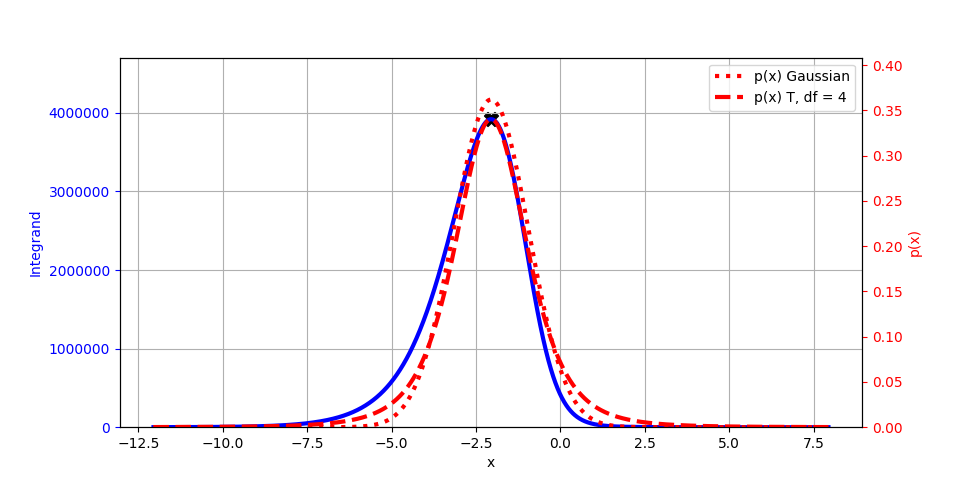
\includegraphics[width=.8\textwidth]{Chap4_ComputationOfIntegral/variance_analysis.png}
\caption{An example integrand function of a model (in blue), and 2 candidate sampling distributions (Gaussian and T) in red.}
\label{fig:Variance_analysis_1}
\end{center}
\end{figure}

\begin{figure}[H]
\begin{center}
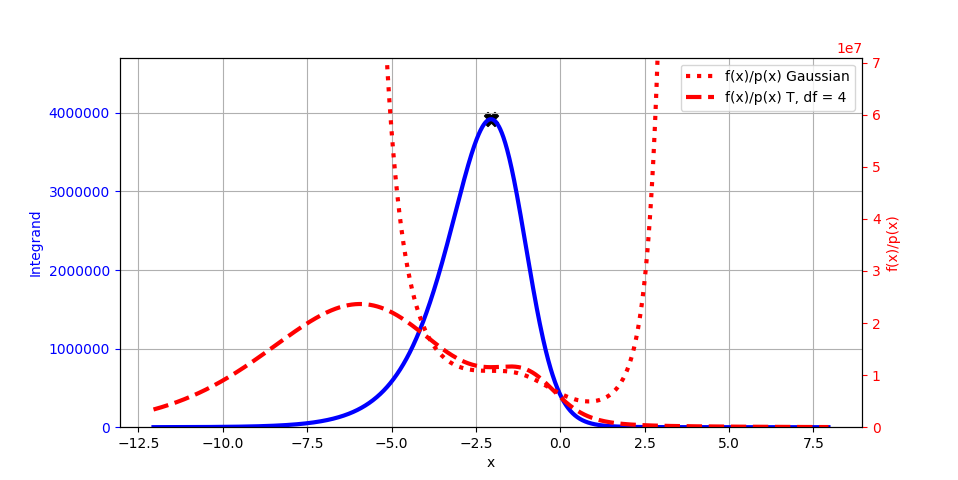
\includegraphics[width=.8\textwidth]{Chap4_ComputationOfIntegral/variance_analysis_2.png}
\caption{An example integrand function of a model (in blue), and the functions \(\frac{f(x)}{p(x)}\) for Gaussian and T distributions. This shows that errors can be greatly magnified under a Gaussian, even when sampling under an important region, while the t-distribution gives a much flatter plot.}
\label{fig:Variance_analysis_2}
\end{center}
\end{figure}

The Gaussian is a very light-tailed distribution, which generally leads to the above behaviour of \(f(\mathbf{x})/p(\mathbf{x})\). A more popular choice is to use the multivariate t-distribution which decay as \((1 + \left\lVert \mathbf{x-\hat{x}} \right\rVert^2 )^{-(\nu + d)/2} \approx \left\lVert \mathbf{x-\hat{x}} \right\rVert ^{-\nu - d} \) asymptotically for large \(x_i\), for a given degree of freedom \(\nu\). Given that \(f(\mathbf{x}) = e^{-Nh(\mathbf{x})}\) decays like \(e^{-\left\lVert \mathbf{x-\hat{x}} \right\rVert}\), any choice of \(\nu\) for the t-distribution will lead to a sampling distribution that has heavier tails than \(f(\mathbf{x})\).
\\\\
For the case of using the t-distribution with degree of freedom \(\nu\) the weights can be calculated:
\begin{empheq}[box=\mymath]
    {equation} 
    w(\mathbf{x}_i) = \frac{1}{p(\mathbf{x}_i)} = \sqrt{\frac{(\nu \pi)^p}{|\mathbf{A}|}} \frac{\Gamma[(\nu+p)/2]}{\Gamma(\nu/2)}  \bigg[ 1 + \frac{1}{\nu} (\mathbf{x}_i - \mathbf{\hat{x}})^T \mathbf{A} ((\mathbf{x}_i - \mathbf{\hat{x}}) \bigg] ^ {\frac{(\nu+p)}{2}} 
\end{empheq}


\subsection{Variance Cancellation}

Variance cancellation occurs when computing a number that is the difference of two approximated, much larger numbers. This phenomenon is of interest in the case of computing the normalizing constant in multi-server node networks. One type of integral of interest that is in the aim of this project to compute, takes the following form:
\begin{equation} \label{eq:summation_first_general_form}
    I = I \Delta = \int_{\mathbb{R}^K} f^{(+)}(\mathbf{x}) - f^{(-)}(\mathbf{x}) d \mathbf{x}
\end{equation}

This can also be written:
\begin{equation} \label{eq:integral_first_general_form}
\begin{split}
    I = \Delta I & = \int_{\mathbb{R}^K} f^{(+)}(\mathbf{x}) d \mathbf{x} - \int_{\mathbb{R}^K} f^{(-)}(\mathbf{x}) d \mathbf{x}\\
    & = I^{(+)} - I^{(-)}
\end{split}
\end{equation}
Where \(f^{(+)}(\mathbf{x})\) and \(f^{(-)}(\mathbf{x})\) are non-negative everywhere, and \(I^{(+)} \approx I^{(-)}\), and \(I\) is of much smaller magnitude than \(I^{(+)}\) and \(I^{(-)}\).
\\\\
This is the form of the multi-server node network integrals, where equation (\ref{eq:integral_first_general_form}) corresponds to the first form of the normalizing constant integral:
\[
G_\theta(\mathbf{N}) = \frac{1}{\prod_{r=1}^R N_r!} \sum_{\mathbf{0 \leq v <s}} \mathbf{\alpha_v} \boldsymbol{\Delta}_{t_0}^{N-v} \boldsymbol{\Delta}_{\mathbf{t}}^{\mathbf{v}} \bigg( \int_{\mathbb{R}^K} e^{-h(\mathbf x, t_0, \mathbf{t})} d \mathbf{x} \bigg)
\]
And equation (\ref{eq:summation_first_general_form}) corresponds to the second form of the normalizing constant integral.
\begin{equation}\label{eq:summation_first_NC_form}
    G_\theta(\mathbf{N}) = \int_{\mathbb{R}^K} \bigg( \frac{1}{\prod_{r=1}^R N_r!} \sum_{\mathbf{0 \leq v <s}} \mathbf{\alpha_v} \boldsymbol{\Delta}_{t_0}^{N-v} \boldsymbol{\Delta}_{\mathbf{t}}^{\mathbf{v}} e^{-h(\mathbf x, t_0, \mathbf{t})}  \bigg) d \mathbf{x}
\end{equation}

Where terms inside the difference \(\boldsymbol{\Delta}\) operators are subtracted to obtain a difference. \(h(\mathbf{x}, t_0, \mathbf{t})\) is given by equation(\ref{eq:log_integrand_x_int_first}). 
\\\\
Now if we restrict ourselves to computing the integrals \(I=\int_{\mathbb{R}^K} f(\mathbf{x}) d\mathbf{x}\) via monte carlo integration, and importance sampling, we can only obtain an approximation of the integral \(\widetilde{I}\). This approximation will have an expectation and variance associated with it. In the case of computing a quantity from the difference of two such integrals \(\widetilde{I}^{(+)}\) and \(\widetilde{I}^{(-)}\). 
\\\\
If we assume the estimates \(\widetilde{I}^{(+)}\) and \(\widetilde{I}^{(-)}\) are independently distributed, and uncorrelated, and have expectations and variances:
\[\mathbb{E}[\widetilde{I}^{(+)}] = I^{(+)} \quad Var[\widetilde{I}^{(+)}] = \sigma^{(+)} = \frac{1}{N} Var \bigg[ \frac{ f^{(+)}(\mathbf{x}) }{ p^{(+)}(\mathbf{x})} \bigg] \]
\[\mathbb{E}[\widetilde{I}^{(-)}] = I^{(-)} \quad Var[\widetilde{I}^{(-)}] = \sigma^{(-)} = \frac{1}{N} Var \bigg[ \frac{ f^{(-)}(\mathbf{x}) }{ p^{(-)}(\mathbf{x})} \bigg] \]
Then the difference of the estimates \(\widetilde{\Delta I}\) must be:
\[\mathbb{E}[\widetilde{\Delta I}] = I^{(+)}-I^{(-)} \quad Var[\widetilde{\Delta I}] = \sigma^{(+)} + \sigma^{(-)} \]
In cases where \(p^{(+)}(\mathbf{x}) \approx p^{(-)}(\mathbf{x}) \approx p(\mathbf{x})\) everywhere:
\[\mathbb{E}[\widetilde{I}] \approx \mathbb{E} \bigg[ \frac{ f^{(+)}(\mathbf{x}) - f^{(-)}(\mathbf{x})}{ p(\mathbf{x})} \bigg]\]

Given a model, the number of intergation samples \(N\) would usually be adjusted to to give an appropriate variance below a certain threshold of the expected value, say \(Var[\widetilde{I}^{(+)}] = \delta \mathbb{E}[\widetilde{I}^{(+)}]\), for small \(\delta\). However, the value of \(N\) that might give a good estimate for \(I^{(+)}\) and \(I^{(-)}\), might be inappropriate for \(I \ll \delta\mathbb{E}[\widetilde{I}^{(+)}]\), since now:
\begin{empheq}[box=\mymath]{equation}
    Var[\widetilde{\Delta I}] = \delta\mathbb{E}[\widetilde{I}^{(+)}] + \delta\mathbb{E}[\widetilde{I}^{(-)}] \gg \mathbb{E}[\widetilde{\Delta I}] = I    
\end{empheq}


This results in what can be regarded as a cancellation by variance, in which case the result gets lost in the variance of its intermediate constituents. In general, it is difficult to estimate the number of samples \(N\) in order to ensure that catastrophic variance cancellation does not occur. It is therefore highly recommended to compute an approximation of \(I\) by computing \(\widetilde{I\Delta}\) in equation (\ref{eq:summation_first_general_form}), if possible, as this does not suffer from the same problems as computing \(\widetilde{\Delta I}\). This motivates the use of method 2, and the form of the integral in (\ref{eq:summation_first_NC_form}) to calculate the normalizing constant.
\\\\
Some numerical experiments to illustrate this phenomenon were also carried out, and are described in section \ref{sec:Multiserver}.

\section{Putting it All Together - The Logistic Sampling Algorithm} \label{sec:put_all_together}
The final algorithm involves the following steps:
\begin{itemize}
    
    \item \textbf{Step 0: Identify model} Given a model of a network to analyze, classify problem one of the following:
        \begin{itemize}
            \item \textit{Case 1}: Single server nodes only
            \item \textit{Case 2}: Single server and delay(infinite server) nodes only
            \item \textit{Case 3}: Multi-server nodes
        \end{itemize}
    
    \item \textbf{Step 1: Choose integrating function} Given a network to analyze, choose from 1 of 3 logistic integrands \(e^{f(\mathbf{x})}\): equation (\ref{eq:log_integrand_single_server}) for networks of case 1, (\ref{eq:log_integrand_infinite_server}) for networks of case 2, 
    (\ref{eq:log_integrand_multi_server_2}) for networks of case 3.
    
    \item \textbf{Step 2: Solve for stationary point} Use an iterative equation (equation (\ref{eq:single_server_stat_pt_equation}) for case 1 and (\ref{eq:inf_server_stat_point}) for case 2), or gradient descent with equation (\ref{eq:multiserver_gradient}) for a general multi-server node network  - case 3, to find the unique stationary point of the integrand function \(\mathbf{\hat{x}}\).
    
    \item \textbf{Step 3: Calculate hessian} Using one of equations (\ref{eq:single_server_hessian_exp}) for case 1, (\ref{eq:inf_server_hessian}) for case 2, or (\ref{eq:multiserver_hessian}) for case 3, compute the Hessian \(\mathbf{A}\) at the stationary point \(\mathbf{\hat{x}}\).
    
    \item \textbf{Step 4: Integrate}. Sample \(N\) points \(\mathbf{x}\) from a t-distribution with mean \(\mathbf{\hat{x}}\), covariance \(\mathbf{A}^{-1}\), and an appropriate degree of freedom \(\nu\), and compute the approximate integral:
    \[\tilde{I} = \frac{1}{N} \sum_{i=1}^N \frac{e^{-f(\mathbf{x}_i)}}{p(\mathbf{x}_i)} \]
    
\end{itemize}
